\section{Gate Closure Phase Diagrams}
\label{sec:results-phase}

Figure~\ref{fig:gate-phase} shifts the discussion from a single robust coarse variable to full gate families under stress. The point of the figure is not that logic is either present or absent, but that closure occupies regimes. The frozen phase bundle spans a \(108\)-row grid over gate family, staging barrier, evaluation horizon \(\tau\), and output-noise level \(p_{\mathrm{gate}}\). For each condition it records three diagnostics on the same frozen data asset: truth error relative to the intended one-step gate, conditional entropy \(H(\mathrm{out}\mid\mathrm{in})\), and route mismatch on the output-bit lens. Taken together, these panels show that familiar truth tables do not all fail in the same way, and that different diagnostics reveal different modes of nonclosure.

\begin{figure}[t]
    \centering
    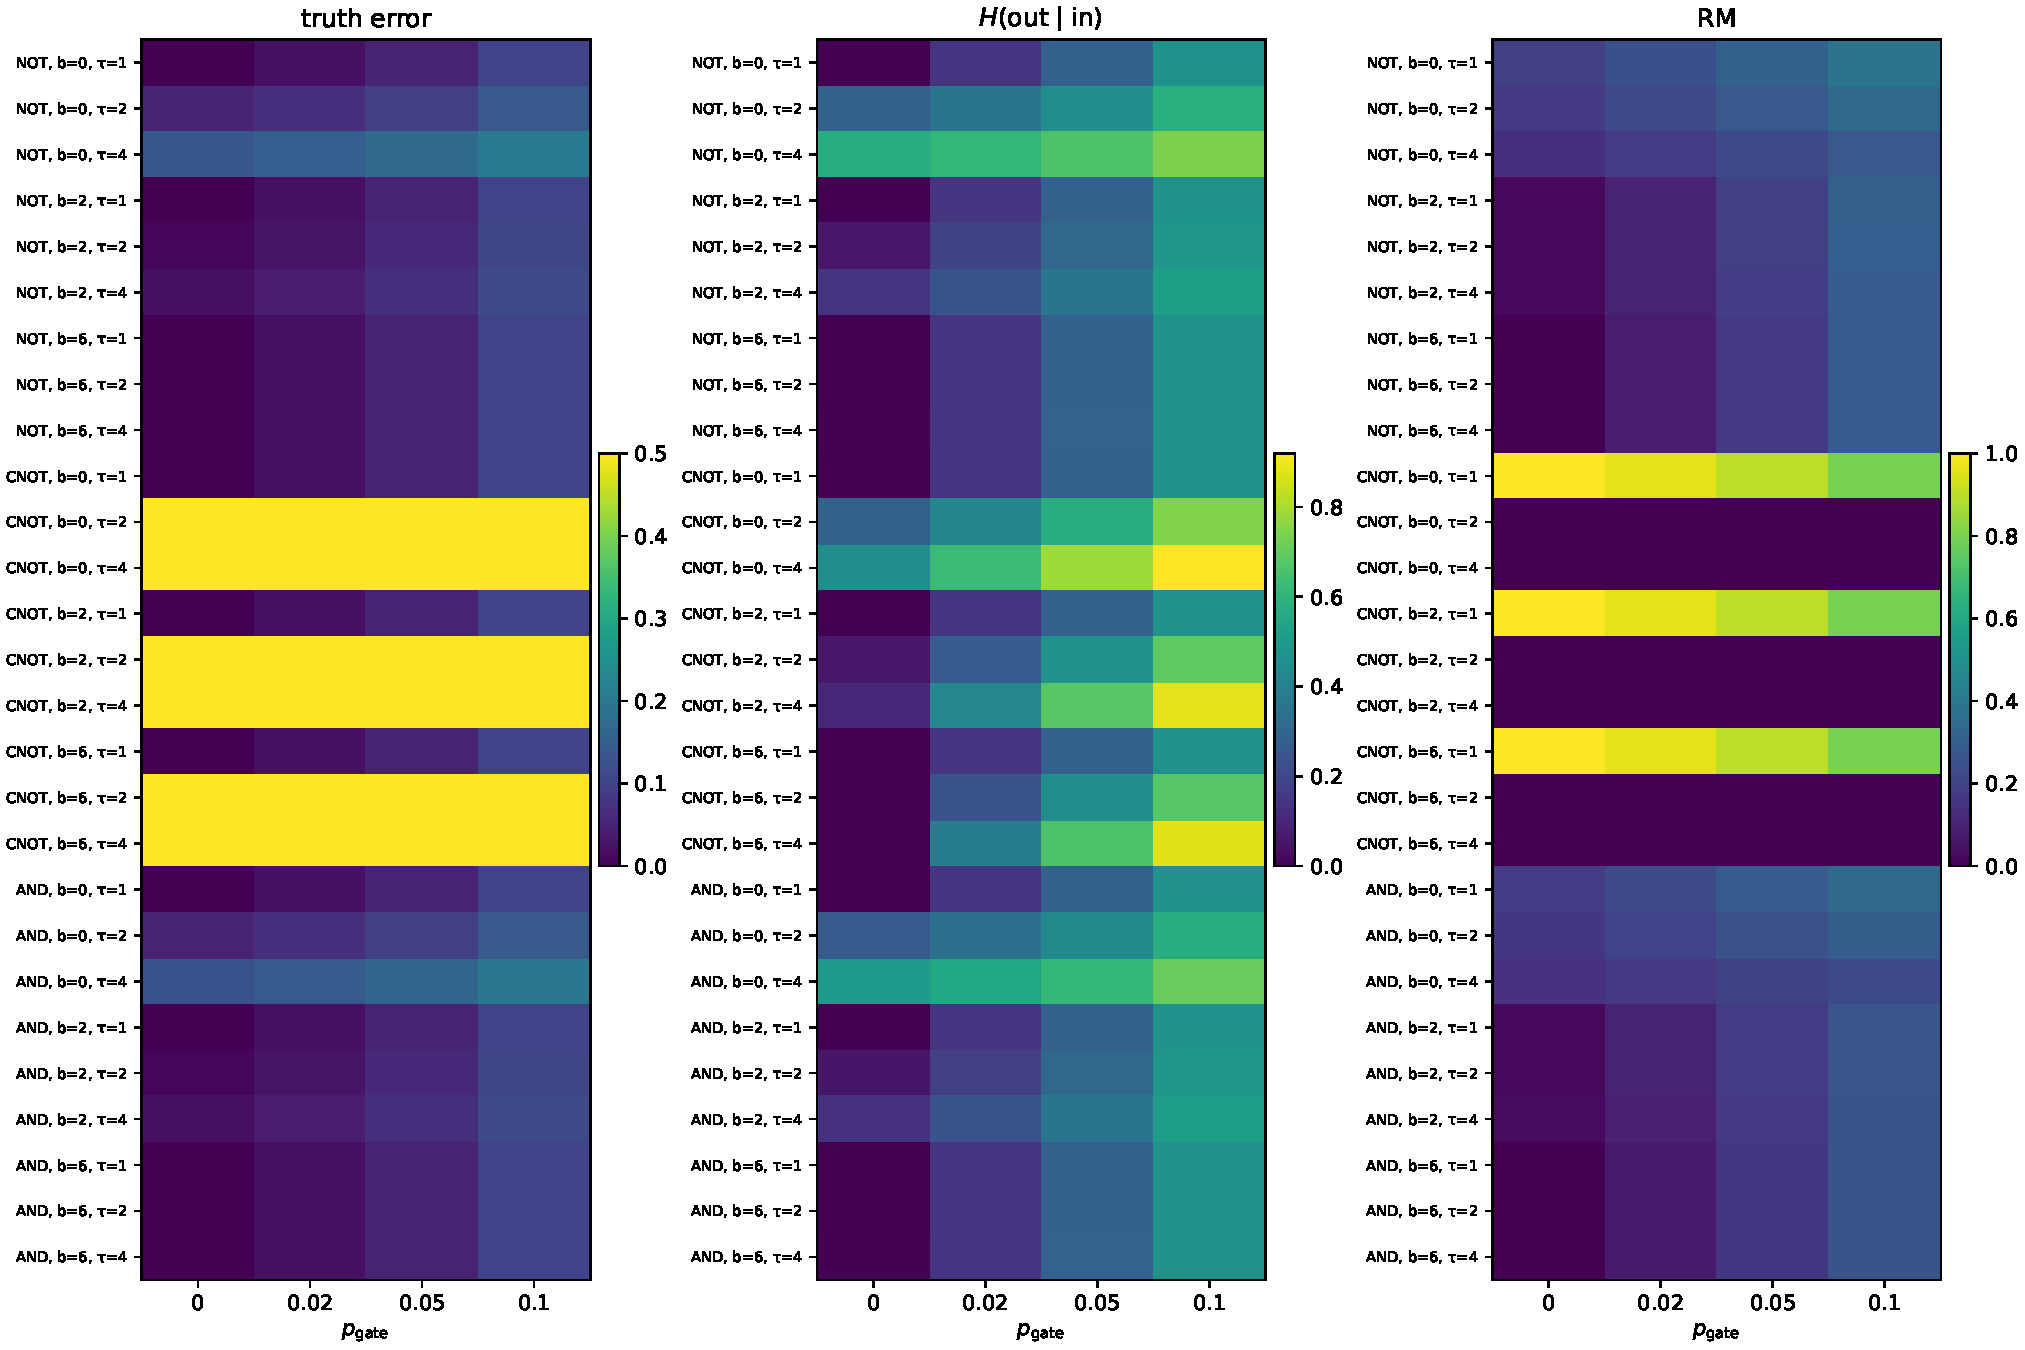
\includegraphics[width=\linewidth]{figures/gate_phase.pdf}
    \caption{Gate-closure phase portrait rendered directly from \protect\path{results/final_claims/figure_gate_phase.csv}. Each row corresponds to a specific gate, barrier, and timescale \(\tau\), while the columns scan output noise \(p_{\mathrm{gate}}\). The three panels report truth error, conditional entropy, and route mismatch on the output-bit lens. The figure is a frozen export of the full \(108\)-row phase bundle.}
    \label{fig:gate-phase}
\end{figure}

At the coarsest level, the frozen bundle shows a clean monotonic trend in truth error with increasing output noise and no anomaly rows. Averaging over barrier and \(\tau\), the NOT truth error rises from \(0.0236\) at \(p_{\mathrm{gate}}=0\) to \(0.1189\) at \(p_{\mathrm{gate}}=0.1\). AND rises from \(0.0225\) to \(0.1180\). CNOT rises from \(0.3333\) to \(0.3667\). These averages are useful as a synopsis, but Figure~\ref{fig:gate-phase} also makes clear why averages alone are insufficient: barrier and horizon matter almost as much as gate noise, and the three diagnostics do not move together in the same way for all gates.

For NOT and AND, the intended gate is recovered cleanly when staging is strong and the evaluation window is short. At barrier \(6\), \(\tau=1\), and \(p_{\mathrm{gate}}=0\), both gates are exact at the channel level in the frozen bundle. NOT records \(\mathrm{err}_{\mathrm{truth}}=0\), \(H(\mathrm{out}\mid\mathrm{in})=0\), and \(\mathrm{RM}=0.000496\). AND records \(\mathrm{err}_{\mathrm{truth}}=0\), \(H(\mathrm{out}\mid\mathrm{in})=0\), and \(\mathrm{RM}=0.000496\). Once the horizon is extended under weak staging, however, closure degrades even when output noise is absent because the stable input bits themselves begin to wander. At barrier \(0\), \(\tau=4\), and \(p_{\mathrm{gate}}=0\), NOT rises to error \(0.1355\), entropy \(0.5723\), and RM \(0.1385\); AND rises to error \(0.1263\), entropy \(0.4974\), and RM \(0.1419\). The symbolic form of the gate has not changed, but the regime in which it is being evaluated has: carrier stability and closure have become the limiting factors.

CNOT behaves differently because the plotted closure lens is intentionally incomplete. At \(\tau=1\) and \(p_{\mathrm{gate}}=0\), the one-step reversible XOR embedding is exact as a gate channel: for barrier \(6\), the frozen bundle records \(\mathrm{err}_{\mathrm{truth}}=0\) and \(H(\mathrm{out}\mid\mathrm{in})=0\). But the RM of the output-bit lens is simultaneously maximal, \(\mathrm{RM}=1\). This is not a contradiction. It is evidence that the output bit alone is not a closed state description for CNOT because its future depends on the retained control bit. The reversible two-bit gate is orderly at the full carrier level, while the one-bit output lens by itself is non-Markovian. CNOT therefore separates channel fidelity from closure in a way that NOT and AND do not.

That separation becomes even sharper at longer horizons. For CNOT, the \(\tau>1\) rows are best read as closure stress tests rather than as repeated grading of the same static truth table. A second noiseless CNOT application toggles the target again, so the one-step XOR truth table is no longer the correct target at \(\tau=2\). This is exactly what appears in the frozen bundle. At barrier \(6\), \(\tau=2\), and \(p_{\mathrm{gate}}=0\), the truth error jumps to \(0.5\), yet the induced error is only \(0.000124\), the conditional entropy is \(0.0018\), and the RM collapses to \(5.55\times 10^{-17}\). At \(\tau=4\), the same pattern persists, with truth error \(0.5\), induced error \(0.000248\), entropy \(0.0033\), and RM \(2.22\times 10^{-16}\). The message is not that CNOT ceases to be structured. The message is that the relevant macro-operator has changed with the protocol horizon. Evaluating \(\tau>1\) as a closure stress test rather than as a truth-table scorecard is therefore essential.

The figure as a whole should be read as a phase portrait of embodied logic. Output noise raises channel error in the expected way, but staging barriers and evaluation horizons determine whether that noise is the dominant failure mode or merely one contributor among several. For NOT and AND, the central transition is from a short-horizon, high-barrier regime in which the gate practically closes, to a longer-horizon, weak-staging regime in which memory corruption drives both entropy and mismatch upward. For CNOT, the key lesson is different: closure depends on retaining the right carrier set. A reversible two-bit gate can be channel-perfect at one horizon while its one-bit output lens remains maximally unclosed.

This regime-based reading sets up the accounting comparison in the next section. The phase portrait already suggests that reversible embedding and erased output are not equivalent descriptions of the same logical object. Section~\ref{sec:results-reversible} makes that distinction explicit by comparing the retained CNOT view and the erased XOR view inside the same underlying laboratory.
